\documentclass[spanish,12pt, a4paper,twoside]{paper}

\let\oldsection\section
\def\section{\cleardoublepage\oldsection}

\usepackage{afterpage}

\usepackage[dvipsnames]{xcolor}

\newcommand\blankpage{%
\null
\thispagestyle{empty}%
\addtocounter{page}{-1}%
\newpage}

%\renewcommand{\listoftables}{Índice de tablas}
\newcommand{\refcruzada}[2]{\hyperref[#2]{#1~\ref{#2}}}

\newcommand*{\NOTE}[1]{\textcolor{ForestGreen}{#1}}

\renewcommand{\labelitemi}{$\square$}
\renewcommand{\labelitemii}{$-$}
\renewcommand{\labelitemiii}{$\bullet$}
\renewcommand{\labelitemiv}{$\ast$}


\makeatletter
\def\namedlabel#1{\begingroup
\def\@currentlabel{#1}%
\@currentlabel
\phantomsection\label{item:\@currentlabel}\endgroup
}
\makeatother


\usepackage[textwidth=15cm, textheight=22.5cm, top=3.5cm, bottom=3.5cm,left= 4cm,right=2cm]{geometry}


\usepackage[spanish]{babel}
\usepackage[utf8]{inputenc}

\usepackage{graphicx}
\usepackage{graphics}
\usepackage{subfigure}
\usepackage{amsmath,amssymb}
\usepackage{float}
\usepackage{changepage}
\usepackage{subcaption}

\usepackage{enumitem}

\usepackage{algorithm}
\usepackage{multirow}

\usepackage[]{hyperref}
\usepackage[T1]{fontenc}
\hypersetup{
backref,
bookmarksnumbered=true,
bookmarksopen=true,
bookmarksopenlevel=1,
colorlinks=false,
%pdfpagemode=UseOutlines,    % this is the option you were lookin for
%pdfpagelayout=TwoPageRight
}
% !TeX spellcheck = es_ES

\begin{document}
    %\maketitle
    %\thispagestyle{empty}
    \begin{titlepage}

        \newcommand{\HRule}{\rule{\linewidth}{0.5mm}} % Defines a new command for the horizontal lines, change thickness here

        \center % Center everything on the page

        %	HEADING SECTIONS
        
\includegraphics[width=2.25cm]{recursos/logoFi.png}
        \hspace{8cm}
        
\includegraphics[width=2cm]{recursos/logoupm.png}
        \\[1cm]

        \textsc{\Large Escuela Técnica Superior de Ingenieros Informáticos}\\[0.5cm]
        \textsc{\large Universidad Politécnica de Madrid}
        \\[3cm]


        %	TITLE SECTION
        \HRule \\[0.4cm]
        { \huge \bfseries serdfgvesrdfserdzfesrdgf}\\[0.4cm] % Title of your document
        \HRule \\[2.5cm]

        \textsc{\LARGE yudtryutyu6ydrujfghdtyju}\\[0.5cm]
        \textsc{\Large dtyjhgftyghujbft yrf ghjdry tjghf }\\[2.5cm]

        %	AUTHOR SECTION
        \begin{flushright}
            \large
            AUTOR: Sergio Flórez Vallina\\
            TUTORES: Alfonso Mateos Caballero y \linebreak
            Antonio Jiménez Martín
        \end{flushright}

        \vspace{1.3cm}

        %	DATE SECTION
        { {2019}}\\[3cm]
        %	LOGO SECTION

        \vfill
        % Fill the rest of the page with whitespace

    \end{titlepage}

    \afterpage{\blankpage}
    \pagenumbering{roman}


    %	AGRADECIMIENTOS
    \section*{AGRADECIMIENTOS}
    Agradezco especialmente a Tino Tello Caballo por toda su paciencia y tiempo para ayudarme
    a dar vida a éste proyecto.

    %	RESUMEN
    \section*{RESUMEN}
    Extensin mxima de una pgina


    %	SUMMARY
    \section*{SUMMARY}
    Extensión máxima de una página


    %	ÍNDICE
    \tableofcontents % indice de contenidos



    %	INDICE DE FIGURAS Y TABLAS
    \listoffigures

    \listoftables

    %	CAPTULOS DEL TRABAJO FIN DE MSTER
    \newpage
    \pagenumbering{arabic}

    %
    % EN ESTE DOCUMENTO ESTÁ EL RESTO DE LA PLANTILLA
    % \section{INFORMACIÓN SOBRE EL TFM}

\subsection{Asignación de Trabajo Fin de Máster}
\noindent El proceso de asignacin de Trabajo Fin de Máster, aprobado por la CAMIA en su novena reunión ordinaria de 15/12/2011, es el siguiente:
\begin{enumerate}
	\item Los alumnos pueden contactar con los profesores del MUIA y acordar el tema de su Trabajo Fin de Mster.
	\item A travs de una aplicacin informtica desarrollada por el DIA (manual de usuario), los alumnos pueden introducir sus preferencias sobre las propuestas de TFM que anualmente realizan por los profesores del MUIA (entre Diciembre y Enero). Identifican, si as lo desean, en orden hasta un mximo de 5 propuestas que ms le atraigan.
	\item En el caso de que no les atraiga ninguna oferta, o no se le haya asignado ninguna de las seleccionadas (varios alumnos pueden seleccionar la misma propuesta), el alumno deber realizar una propuesta, encuadrndola en una de las materias del MUIA e indicando hasta tres profesores de la misma que puedan ejercer de directores.
\end{enumerate}

En el siguiente enlace (http://www.dia.fi.upm.es/grupos-investigacion) se dispone de un listado de los grupos de investigacin, con una descripcin breve de los mismos y enlaces a sus correspondientes pginas web.

Los alumnos pueden identificar a partir de la informacin proporcionada por los grupos de investigacn la lnea en que basar el desarrollo de su TFM e incluso de una posterior Tesis Doctoral.

Se permitide un TFM por dos profesores, previa solicitud y justificac de la misma a la CAMIA, siendo obligatorio que al menos uno de los dos profesores forme parte del profesorado del ter.

La  asigne Trabajos Fin de Master se encuentra disponible en la web.



\subsection{Tribunal evaluador}
\noindent Se constituiun tribunal para cada defensa de TFM. El director del TFM formarte del tribunal y eleg miembros restantes, debiendo ser:
\begin{itemize}
	\item Uno de ellos, un profesor del MUIA de la materia del TFM.
	\item  El otro, un profesor del MUIA de la materia del TFM o de una mater.
\end{itemize}

En caso de codireccionesl visto bueno.


\subsection{Proceso administrativo de defensa del TFM}
\noindent La Figura \label{fig:proceso} muestra el proceso completo desde la asignacer (TFM) hasta su defensa.

\begin{figure}[h]
	\centering
	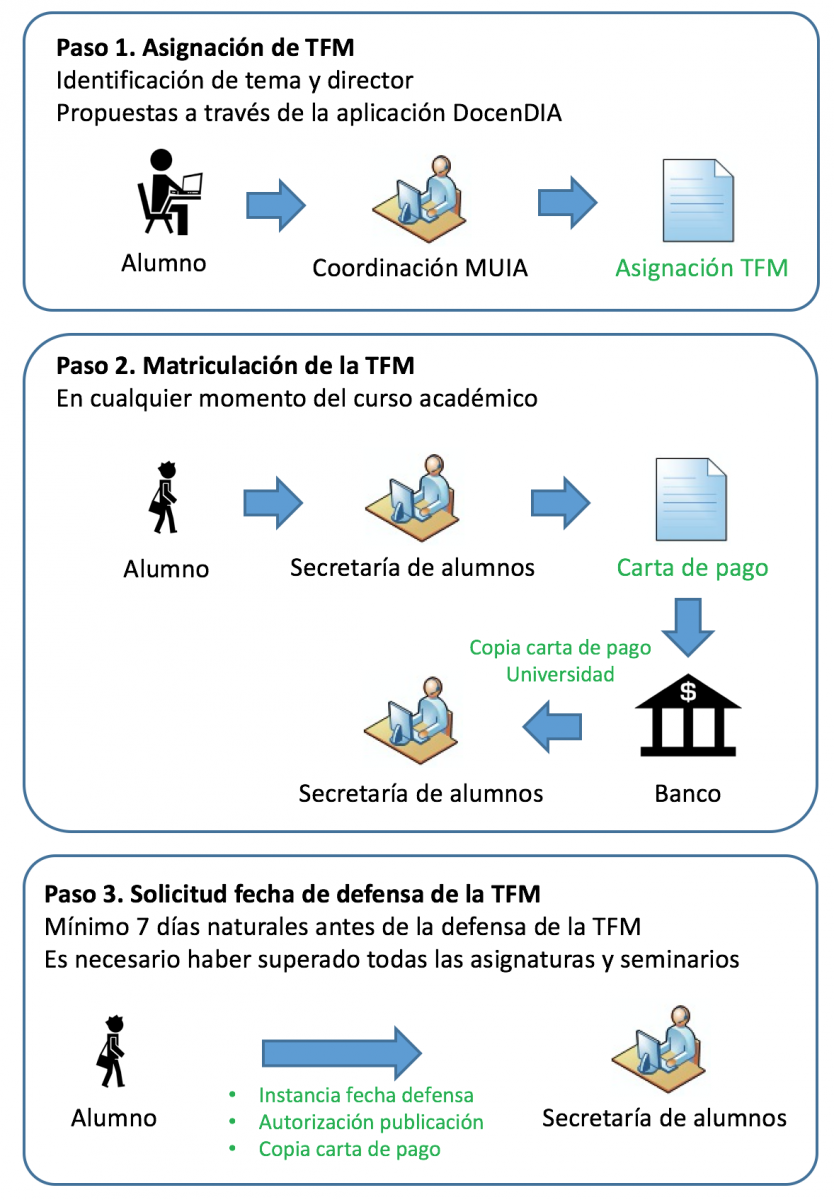
\includegraphics[width=0.65\textwidth]{recursos/Proceso}
	\caption{Proceso desde la asignahasta la defensa del TFM}
	\label{fig:proceso}
\end{figure}


El TFM {\bf puede matricularse en cualquier momento a lo largo del curmico} en la Secreta alumnos (ETSIInf), donde se generarcarta de pago.

El tiempo que puede transcurrir entre la matriculla defensa del TFM no  limitado (salvo los 7  naturales de antelaccircunscrito al mismo curso .

Es necesario tener en cuenta que al hacer el pago, el importe de la  que llegue a la Universidad tiene que coincidir exactamente con el de la carta de pago. Si no hay coincidencia no se  defender hasta que esa cantidad coincidiera, por lo que las comisiones bancarias o cargos correspondientes transferencias desde el extranjero, cambios de divisas, etc. los tiene que asumir el alumno. Una vez realizado el pago se debe entregar en el Centro de Postgrado (o bien enviarlos mediante un mail a centro.postgrado@fi.upm.es) lo siguiente:

\begin{itemize}
	\item el resguardo de la transferencia.
	\item y los datos siguientes:     
	\begin{itemize}
		\item Nombre y apellidos de la persona matriculada.
		\item Nombre del Master.
		\item Fecha de pago.
		\item Cantidad transferida.
		\item Cuenta desde la que se transfiere la cantidad.
	\end{itemize}
\end{itemize}

{\bf Nota:} El alumno debe tener en cuenta que si no  matriculado de ninguna asignatura en el MUIA pierde su  oficial con la UPM y no puede optar a becas oficiales y no oficiales,  Por ello, recomendamos a los alumnos que  tengan pendiente el TFM la matriculen al principio del semestre correspondiente para mantener la  con la universidad.

Las {\bf defensas} de los TFM se  realizar a lo largo de todo el curso

Una vez matriculada el TFM, el alumno  con una {\bf  de 7  naturales} la fecha y tribunal de la defensa, mediante la instancia correspondiente, en la {\bf  que se debe entregar es la siguiente:
	
	\begin{itemize}
		\item Instancia con tribunal y fecha de la defensa del TFM y  del director/es.
		\item Copia de la carta de pago de  del TFM.
		\item Instancia de  de cara a que el TFM pueda ser publicada en el archivo digital de la UPM.
	\end{itemize}
	a de la misma un ejemplar del TFM en el formato prescrito en formato  (pdf).
	
	El secretario del tribunal l encargado de {\bf reservar hemiciclo} para la  del acto de defensa del TFM y de {\bf recoger y entregar las actas} de la defensa en la  de Postgrado de la ETSIInf.
	
	\subsection{Acto de defensa del TFM}
	\noindent La {\bf lengua} tanto de la memoria del TFM, como de la defensa del mismo ante el tribunal,  ser el castellano o el .
	
	El secretario del tribunal s de Postgrado de la ETSIInf.
	
	La {\bf defensa del TFM}  oral sobre el misma por parte del alumno durante un {\bf tiempo  de 20 minutos y  de 20 minutos.
		
		El tribunal  los siguientes aspectos a la hora de evaluar el TFM:
		\begin{itemize}
			\item El alumno {\bf conoce}  de Inteligencia Artificial que le permiten abordar y solucionar problemas de .
			\item El alumno {\bf aplica}  existentes de la Inteligencia Artificial para la  de un problema.
			\item El alumno {\bf crea} alguna  de  de la Inteligencia Artificial.
			\item El alumno {\bf crea y difunde}  aceptados) los resultados de la TFM en una revista o congreso (nacional o internacional) con  por pares.
		\end{itemize}
		
		
		
		\subsection{Confidencialidad}
		\noindent En el caso de que el alumno desee la confidencialidad sobre su TFM,  solicitarlo mediante la correspondiente instancia disponible en la web que se  con una copia impresa del TFM y se  por Registro en  de Alumnos.
		
		
		\subsection{Concesión de Matriculas de Honor}
		\noindent Para proponer la  de Matrícula de Honor, se  en cuenta los criterios ya aprobados en la CAMIA de 15/12/2012: El alumno {\bf crea y difunde}  o  (nacional o internacional) con  por pares.
		
		formada por 3 profesores del Master Universitario en Inteligencia Artificial (MUIA) para la  aquellos profesores que hayan tutorizado alguna de los TFM propuesta para MH.
		
		Una vez finalizada la defensa de todos los trabajos de fin de  lugar en el mes de Julio. 
		
		La  solamente  en cuenta los TFM que hayan sido propuestas para MH por los respectivos tribunales.
		
		El tribunal otra convocatoria posterior.
		
		Si hubiese un  de alumnos matriculados (de conformidad con lo dispuesto en el Real Decreto 1125/2003, de 5 de septiembre), se  en cuenta las siguientes recomendaciones:
		
		\begin{itemize}
			\item Se  de honor obtenidas por el alumno en asignaturas del master.
		\end{itemize}
		
		
		\section{TABLAS, FIGURAS, EXPRESIONES MATEMÁTICAS Y ALGORITMOS}
		
		\subsection{Figuras}
		
		Las Figuras \ref{fig:Bernoulli1} y \ref{fig:violin_besa_escenario4} muestran ejemplos de  insertar figuras en el TFM.
		\begin{figure*}[htb]
			\centering
			\begin{subfigure}{0.5\textwidth}
				\includegraphics[width=\textwidth]{recursos/Figure1a}
				\caption{Mean cumulative regret along trials}
				\label{fig:Bernoulli1_semilog}
			\end{subfigure}
			\begin{subfigure}{0.5\textwidth}
				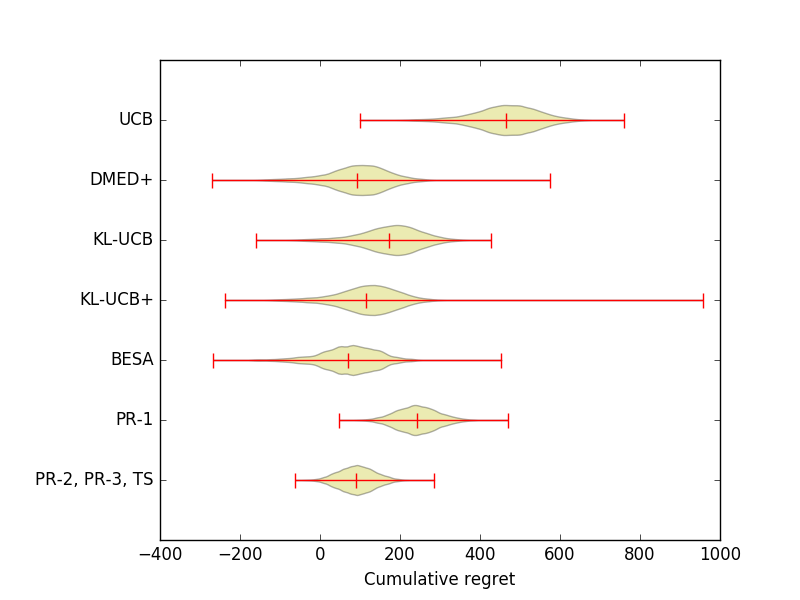
\includegraphics[width=\textwidth]{recursos/Figure1b}
				\caption{Multiple violinplot}
				\label{fig:Bernoulli1_boxplot}
			\end{subfigure}
			\caption{Comparative of the policies for scenario 1}
			\label{fig:Bernoulli1}
		\end{figure*}
		
		\begin{figure*}
			\centering
			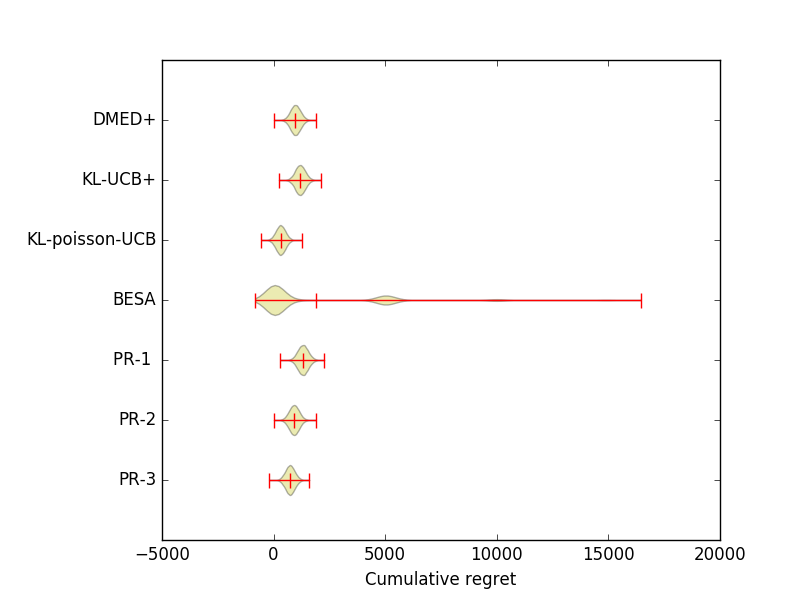
\includegraphics[width=0.5\textwidth]{recursos/Figure2}
			\caption{Violinplot fot BESA in scenario 4}
			\label{fig:violin_besa_escenario4}
		\end{figure*}
		
		
		
		\subsection{Expresiones matemáticas}
		A continuación, se muestran algunos ejemplos de expresiones matemáticas:
		\begin{equation}
		\mu^*\times 25000-\frac{1}{1000}\sum_{r=1}^{1000}\sum_{i=1}^{K}\sum_{j=1}^{25000}\mu_i\times X_{i,j}^r.
		\end{equation}
		
		\begin{equation}
		\mu_{\widetilde{A}}(x)=\left\{ \begin{array}{cc}
		\frac{x-a_{1}}{a_{2}-a_{1}} & if\; a_{1}\leq x\leq a_{2}\\
		1 & if\; a_{2}\leq x\leq a_{3}\\
		\frac{x-a_{4}}{a_{3}-a_{4}} & if\; a_{3}\leq x\leq a_{4}\\
		0 & otherwise
		\end{array}\right. .
		\end{equation}
		
		
		\begin{equation}
		\begin{tabular}{ll}
		$\widetilde{DD}(A_{1},A_{4})$ & $=\widetilde{DD}(A_{1},A_{4}|P_{1})\oplus 
		\widetilde{DD}(A_{1},A_{4}|P_{2})$ \\ 
		$=[\widetilde{dd}(A_{1},A_{2})\otimes \widetilde{dd}(A_{2},A_{4})]\oplus \lbrack \widetilde{dd}(A_{1},A_{3})\otimes \widetilde{%
			dd}(A_{3},A_{4})].$%
		\end{tabular}%
		\end{equation}
		
		
		
		\begin{itemize}
			\item Si$\;{max} \{(a_{4}-a_{1}),(b_{4}-b_{1})\}\neq 0$, entonces
			\begin{eqnarray*}
				{\small S(}\widetilde{A}{\small ,}\widetilde{B}{\small )} &{\small =}&%
				\left. {\small 1-(1-\alpha -\beta })\times \left ( {\small 1-}\frac{\int_{0}^{1}%
					{\small \mu }_{\widetilde{A}\cap \widetilde{B}}{\small (x)dx}}{\int_{0}^{1}%
					{\small \mu }_{\widetilde{A}\cup \widetilde{B}}{\small (x)dx}}\right)
				\right.  \\
				&&\left. -{\small \alpha } \frac{\sum {\small \mid a}_{i}{\small -b}_{i}%
					{\small \mid }}{{\small 4}}-{\small \beta }\frac{{\small d[(X}_{\widetilde{A}%
					}{\small ,Y}_{\widetilde{A}}{\small ),(X}_{\widetilde{B}}{\small ,Y}_{%
						\widetilde{B}}{\small )]}}{{\small M}}\right., 
			\end{eqnarray*}
			
			\item En caso contrario,%
			\begin{eqnarray*}
				{\small S(}\widetilde{A}{\small ,}\widetilde{B}{\small )} &{\small =}&%
				\left. {\small 1-}%
				\left( \frac{{\small 1-\alpha -\beta }}{{\small 2}}{\small +\alpha } \right) \times
				\frac{\sum {\small \mid a}_{i}{\small -b}_{i}{\small \mid }}{{\small 4}}%
				{\small -}\right.  \\
				&&\left. {\small -}\left( \frac{{\small 1-\alpha -\beta }}{{\small 2}}%
				{\small +\beta }\right)\times \frac{{\small d[(X}_{\widetilde{A}}{\small ,Y}_{%
						\widetilde{A}}{\small ),(X}_{\widetilde{B}}{\small ,Y}_{\widetilde{B}}%
					{\small )]}}{{\small M}}\right., 
			\end{eqnarray*}
		\end{itemize}
		donde $\alpha +\beta <1$, $\mu _{\widetilde{\chi }}$ es la funcion de pertenencia de $\widetilde{\chi}$, 
		\begin{equation}
		M=\underset{[0,1]\times[0,\frac{1}{2}]}{max}\{d((x,y),(x^{\prime },y^{\prime }))\}\text{,} 
		\end{equation}%
		\begin{equation*}
		\mu _{\widetilde{A}\cap \widetilde{B}}(x)=\underset{0\leq x\leq 1}{min}%
		\{\mu _{\widetilde{A}}(x),\mu _{\widetilde{B}}(x)\} ,
		\;\;\; \mu _{\widetilde{A}\cup \widetilde{B}}(x)=\underset{0\leq x\leq 1}{max}%
		\{\mu _{\widetilde{A}}(x),\mu _{\widetilde{B}}(x)\}.
		\end{equation*}%
		
		\subsection{Algoritmos}
		
		El Algoritmo \ref{getDelay} ilustra la forma que debe adoptarse. 
		\begin{algorithm}[h]
			%\begin{algorithmic}
			{\bf  Data:} ($t_0$ = instante en el que se genera el retardo)
			\medskip
			
			\hspace{0.5em} {\bf if} $(update\_architecture==1)$ {\bf then} 
			
			\hspace{1.5em} {\bf if} $(delay\_scenario==1)$ {\bf then} delay$=C$
			
			\hspace{1.5em} {\bf else} 
			
			\hspace{2.5em} {\bf if} $(reward\_scenario==1)$ {\bf then} 
			
			\hspace{3.5em} delay $\leftarrow [0,300]$-trunc\_Exp($\lambda=1/80$)
			
			\hspace{2.5em} {\bf else} 
			
			\hspace{3.5em} delay $\leftarrow [0,480]$-trunc\_Exp($\lambda=1/150$)
			
			\hspace{2.5em} {\bf end if}
			
			\hspace{1.5em} {\bf end if}
			
			\hspace{0.5em} {\bf else} (arquitectura en modo batch)
			
			\hspace{1.5em} delay= difference(24:00, $t_0$)
			
			\hspace{0.5em} {\bf end if}
			
			\hspace{0.5em}  {\bf return} delay
			
			{\bf end} 
			\caption{$getDelay(t_0)$}
			\label{getDelay}
		\end{algorithm}
		
		
		\subsection{Tablas}
		Las Tablas \ref{table:results45} y \ref{table:risk} muestran el formato de tabla a utilizar.
		
		\begin{table}[htb]
			\centering
			\caption{Mean cumulative regrets and standard deviations}
			\label{table:results45}
			\begin{tabular}{llllll}
				\hline
				& \multicolumn{2}{c}{\small Truncated Poisson} &  & \multicolumn{2}{c}{\small Truncated Exponential} \\ 
				\cline{2-3}\cline{5-6}\cline{5-6}
				& {\small Mean} & ${\small \sigma}$ &  &  {\small Mean} & ${\small \sigma}$\\ \hline
				{\small UCB}      & {\small 2632.65} & {\small 246.03}  &  & {\small 1295.79} & {\small 514.03}   \\
				{\small DMED+}            & {\small 978.56} & {\small 225.24}  &  & {\bf \small645.70} & {\small 493.8}   \\
				{\small KL-UCB}   & {\small 1817.4} & {\small 236.57}  &  & {\small 1219.98} & {\small 510.69}   \\ 
				{\small KL-UCB poisson}    & {\bf \small314.99*} & {\small 201.79}  &  & {\small -} & {\small -}   \\
				{\small KL-UCB exp}    & {\small -} & {\small -}  &  & {\small 786.30} & {\small 498.16}   \\
				{\small KL-UCB+}    & {\small 1190.64} & {\small 225.82}  &  & {\small 813.45} & {\small 494.59}   \\
				{\small BESA}      & {\small 2015.73} & {\small 3561.5}  &  & {\small 755.87} & {\small 2323.22}   \\
				{\small PR-1}            & {\small 1314.9} & {\small 234.25}  &  & {\small 660.64} & {\small 492.37}   \\ 
				{\small PR-2 (TS)}  & ${\bf 917.67}$ & {\small222.79}  &  & {\bf \small630.38} & {\small487.01} \\
				{\small PR-3}  & ${\bf 736.6}$ & {\small210.96}  &  & {\bf \small565.79*} & {\small480.99} \\
				\hline
			\end{tabular}
		\end{table}
		
		\begin{table}[htb]
			\centering
			\caption{Risks to $A_5$ after the implementation of the selected safeguards }
			\label{table:risk}
			\begin{tabular}{cccc}
				\hline
				\noalign{\smallskip} 
				{\scriptsize{Threat}}& {\scriptsize{Confidentiality}} & {\scriptsize{Integrity}} & {\scriptsize{Authenticity}}\tabularnewline
				\hline  
				{\scriptsize{$T_{1}^{1}$}} & \scriptsize{(16.9, 161.72, 936.2, 3681.5)} & \scriptsize{(32.70, 239.7, 1295.6, 5197.4)} & \scriptsize{(25.1, 198.6, 1576.7, 5777.1)}\\
				{\scriptsize{$T_{1}^{2}$}} & \scriptsize{(0, 49.6, 458.1, 1791.2)} & \scriptsize{(0, 29.7, 289.7, 1397.1)} & \scriptsize{(0, 24.6, 352.6, 1552.9)}\\
				{\scriptsize{$T_{2}^{2}$}} & \scriptsize{(0, 49.6, 458.1, 1791.2)} & \scriptsize{(0, 29.7, 289.7, 1397.1)} & \scriptsize{(76, 379.3, 2074.3, 5588.4)}\\
				{\scriptsize{$T_{1}^{3}$}} & \scriptsize{(12.2, 110.5, 647.2, 2465.6)} & \scriptsize{(21.9, 147.3, 744.3, 2958.7)} & \scriptsize{(6.8, 58.5, 487.1, 1923.2)}\\ 
				{\scriptsize{$T_{1}^{4}$}} & \scriptsize{(34.8, 245.5, 1176.8, 3793.2)} & \scriptsize{(62.7, 327.4, 1353.3, 4551.9)} & \scriptsize{(19.5, 129.9, 885.7, 2958.7)}\\
				\hline 
			\end{tabular}
		\end{table}
		
		
		\section{CONTENIDOS DEL TFM}
		Durante la resultante de la tesis satisface los deseos o necesidades del cliente (real, potencial o ficticio).
		
		{\bf Conclusiones:}
		Establecer las conclusiones del trabajo  actuales aplicadas al problema, planteando leneas de I+D+i realistas y capaces de superarlos.
		
		\section{CONCLUSIONES Y LENEAS FUTURAS DE TRABAJO}
		Establecer las conclusiones del trabajo apoyándose fundamentalmente en los datos y observaciones obtenidas durante su desarrollo. Discutir que medios, cauces, etapas y tecnologías hartan falta (si procede) para llevar a cabo una implantación real de los resultados.
		Discutir los limites de las tecnologías actuales aplicadas al problema, planteando leneas de I+D+i realistas y capaces de superarlos.
		
		\section{SOBRE LAS REFERENCIAS}
		
		La bibliográfica o referencias deben aparecer siempre al final de la tesis, incluso en aquellos casos donde se hayan utilizado notas finales. La bibliográfica debe incluir los materiales utilizados, incluida la edición, para que la cita pueda ser fácilmente verificada. 
		
		\bigskip
		{\bf Citar dentro del texto:}
		
		Las fuentes consultadas se describen brevemente dentro del texto y estas citas cortas se amplían en una lista de referencias final, en la que se ofrece la información bibliográfica completa. 
		
		La cita dentro del texto es una referencia corta que permite identificar la publicación de donde se ha extraído una frase o parafraseado una idea, e indica la localización precisa dentro de la publicación fuente. Esta cita informa del apellido del autor, la fecha de publicación y la pagina (o paginas) y se redacta de la forma que puede verse a través de los siguientes ejemplos:
		
		Cuando se citan las palabras exactas del autor deben presentarse entre comillas e indicarse, tras el apellido del autor y, entre paréntesis, la fecha de publicación de la obra citada, seguida de la/s pagina/s.
		
		Si lo que se reproduce es la idea de un autor (no sus palabras exactas) no se ponrse; debe indicarse siempre con puntos suspensivos entre corchetes [...]
		
		Ejemplos de como citar una referencia en el texto son los siguientes \cite{Ashtiani2014} o \cite{Ashtiani2014,Mateos2009,Vicente2016}.
		
		
		\bigskip
		{\bf Como ordenar las referencias:}
		\begin{enumerate}
			\item Las referencias bibliográficas deben presentarse ordenadas alfabéticamente por el apellido del autor, o del primer autor en caso de que sean varios.
			\item Si un autor tiene varias obras se orde
			\item Si son trabajos de un autor en colabora de publicación. Las publicaciones individuales se colocan antes de las obras en colaboración.
		\end{enumerate}
		
		\bigskip
		{\bf Como citar un articulo de revista}
		
		Un articulo de revista, siguiendo las normas de la APA, se cita de acuerdo con el siguiente esquema general:
		Apellido(s), Iniciales del nombre o nombres. (Aulo.
		
		\bigskip
		{\bf Cmo citar una monografista/libro}
		
		Las monografistas, siguiendo las normas de la APA, se citan de acuerdo con el siguiente esquema general:
		Apellido(s), n cursiva.
		
		\bigskip
		{\bf Como citar un capitulo de un libro}
		
		Los c Editorial.
		
		\bigskip
		{\bf Cmo citar un acta de un congreso}
		
		Apellido(s), Iniciales del nombre o nombres. (A). Ttulo del trabajo. En A. A. Apellido(s) Editor A, B. B. Apellido(s) Editor B, y C. Apellido(s) Editor C (Eds. o Comps. et.), Nombre de los proceedings en cursiva (pp. xxx-xxx). Lugar de publicaci: Editorial.
		
		\bigskip
		{\bf Como citar tesis doctorales, trabajos fin de míster o proyectos fin de carrera}
		
		Apellido(s), Nombre. (Aro). Titulo de la obra en cursiva. (Tesis doctoral). Institución a académica en la que se presenta. Lugar.
		
		\bigskip
		{\bf Como citar un recurso de Internet}
		
		Los recursos disponibles en Internet pueden presentar una tipografía muy variada: revistas, , portales, bases de datos... Por ello, es muy difícil dar una pauta general que sirva para cualquier tipo de recurso.
		Como mínimo una referencia de Internet debe tener los siguientes datos:
		\begin{enumerate}
			\item Titulo y autores del documento.
			\item Fecha en que se )
		\end{enumerate}
		
		Veamos, a .
		
		Monografistas:
		Se emplea la misma forma de cita que para las monografistas en versión impresa. Debe agregar la URL y la fecha en que se consulta el documento
		
		de revistas:
		Se emplea la misma forma de cita que para los artículos de revista en  impresa. Debe agregar la URL y la fecha en que se  el documento.
		
		de revistas  que se encuentran en una base de datos:
		Se emplea la misma forma de cita que para los  de revista en  impresa, pero debe  el nombre de la base datos, la fecha en que se  el documento.
    %
    %

    \graphicspath{{capitulos/Capitulo1-Introduccion/recursos/}}

\section{Introducción y objetivos}

En éste capítulo describiremos el contexto principal y las hipótesis iniciales de las que parte el proyecto, así como una ligera introducción al problema bajo estudio en el presente proyecto de fin de máster.

\begin{figure}
	\centering
	\includegraphics[width=0.7\linewidth]{Figure1a}
	\caption{ figura de test}
	\label{fig:figure1a}
\end{figure}

    \newpage

	\graphicspath{{capitulos/Capitulo2-Definicion-del-problema/recursos/}}

\section{Definición del problema} \label{apartado:2}

Tal y como se ha introducido antes, el proyecto ABACO pretende automatizar el proceso de creación de un horario de trabajo para
los distintos controladores del espacio aéreo de forma que dada una sectorización del espacio aéreo, todos los sectores puedan ser
controlados.

\subsection{Sectores y sectorización}
En primera lugar, explicaremos brevemente cómo se divide el espacio aéreo del territorio español, cuyo organismo encargado de su gestión es AENA. Si bien la realidad es muy compleja, aquí unicamente describiremos una simplificación de la misma, omitiéndose detalles técnicos de aviación que no son necesarios para la implementación del sistema.
\\

El espacio aéreo mundial se encuentra dividido en \textit{FIR}s (\textit{Flight Information Region}), áreas del territorio sobre las que se mueven los diferentes aviones de cada compañía aérea de cada país, en la \refcruzada{Figura}{fig:fireuropa} puede verse graficamente los límites de cada región. En el caso de España, podemos ver que tiene control sobre 3 \textit{FIR}s: el de Barcelona, el de Madrid y el de Canarias, sin embargo, a nivel nacional, existen algunas subdivisiones denominadas \textit{Dependencias} (ya que dependen del \textit{FIR} en el que se encuentren), que permiten una mejor gestión del territorio:
\begin{itemize}
	\item Barcelona RutaE
	\item Barcelona RutaW
	\item Barcelona TMA ESTE
	\item Barcelona TMA NORTE
	\item Barcelona TMA OESTE
	\item Canarias ACC App
	\item Canarias ACC Ruta
	\item Madrid Ruta 1
	\item Madrid Ruta 2
	\item Madrid TMA NORTE
	\item Madrid TMA SUR
	\item Malaga App
	\item Palma TACC
	\item Sevilla TACC
	\item  Valencia TACC TMA
\end{itemize}

Algunos de ellos aparecerán en los casos de prueba del sistema del \refcruzada{Apartado}{apartado:5}
\begin{figure}
	\centering
	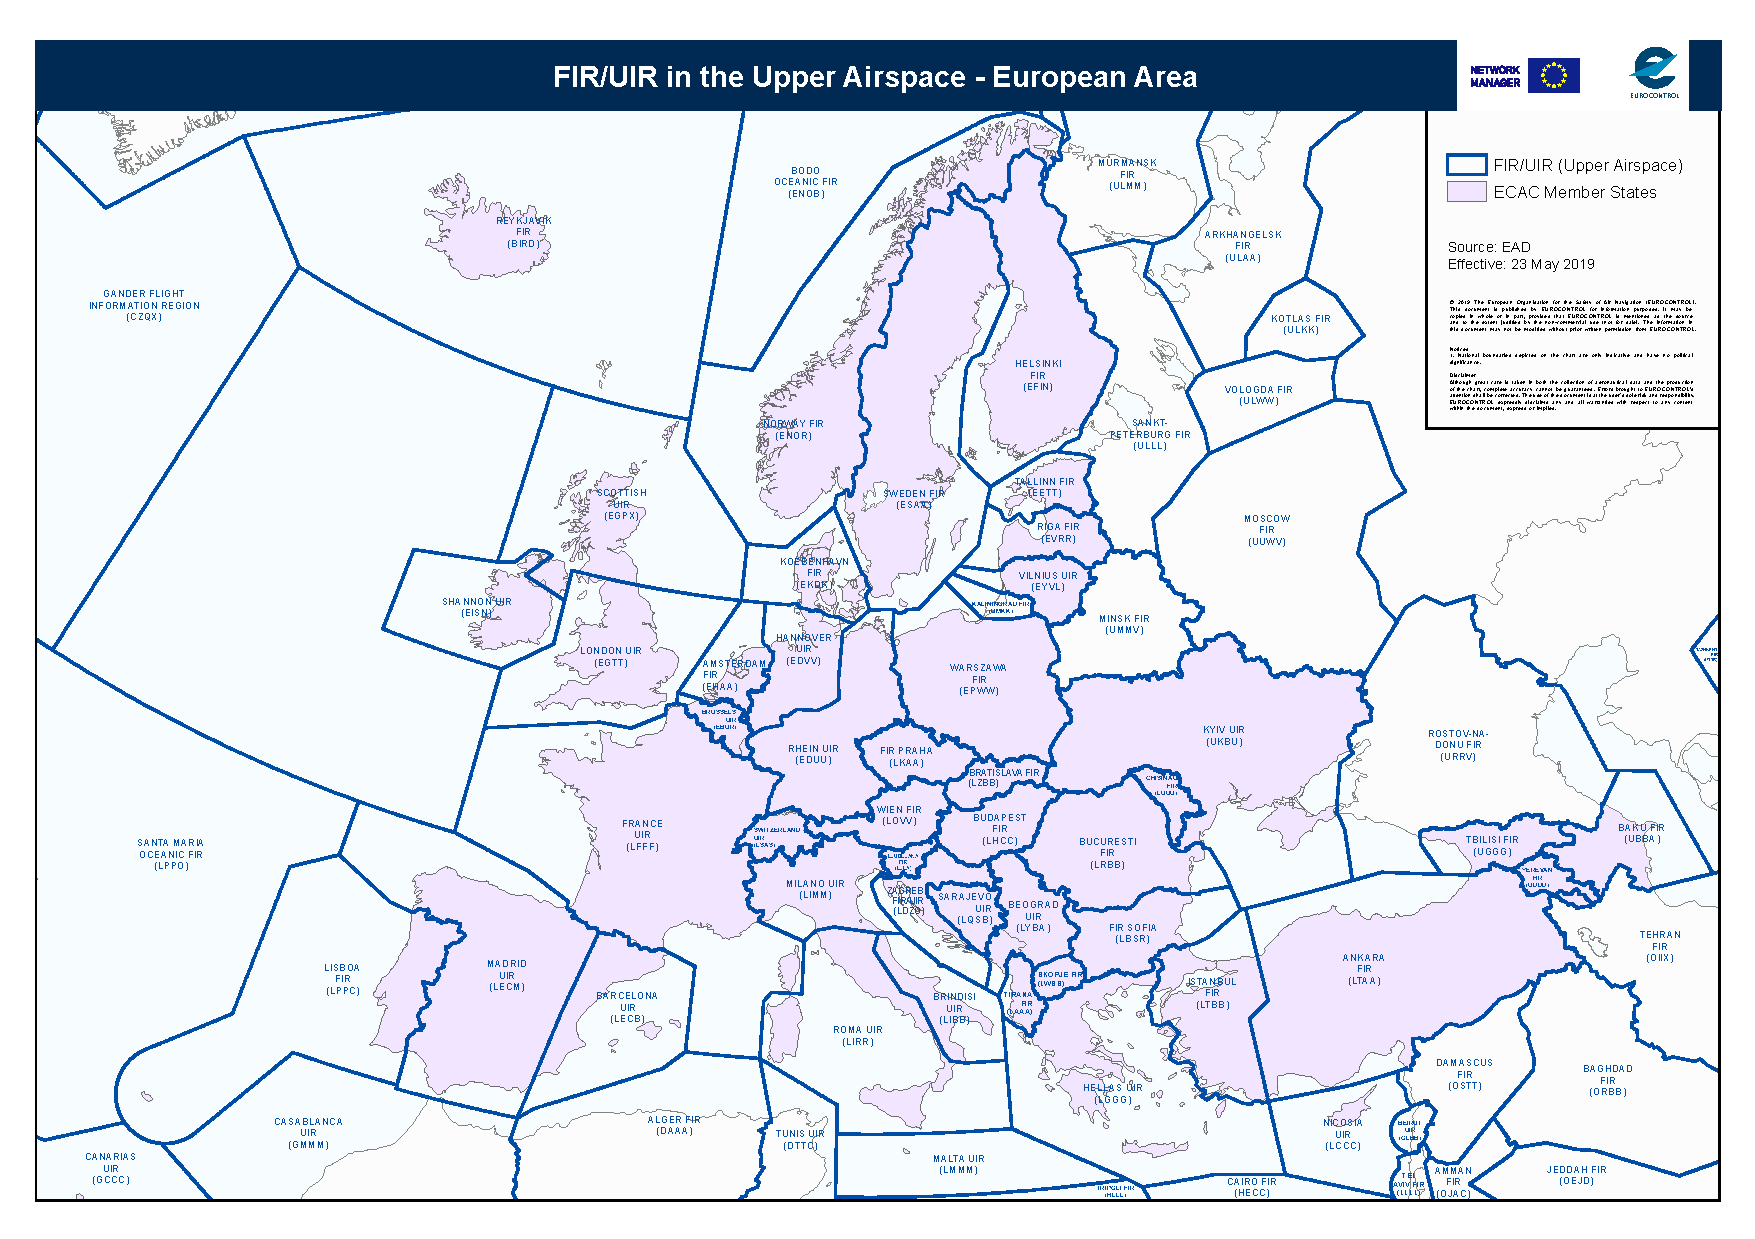
\includegraphics[width=1\linewidth]{capitulos/Capitulo2-Definicion-del-problema/recursos/FIR_europa}
	\caption{FIRs del la zona europea. Fuente: EUROCONTROL}
	\label{fig:fireuropa}
\end{figure}



	\newpage

%	\section{Introducción y objetivos}

En éste capítulo describiremos el contexto principal y las hipótesis iniciales de las que parte el proyecto, así como una ligera introducción al problema bajo estudio en el presente proyecto de fin de máster.

\begin{figure}
	\centering
	\includegraphics[width=0.7\linewidth]{capitulos/Capitulo1/Figure1a}
	\caption{ figura de test}
	\label{fig:figure1a}
\end{figure}

%	\newpage

	%\include{capitulos/CapituloXXX-YYY/CapituloXXX}
    %\newpage

    \section*{ANEXOS}


    %	REFERENCIAS
    \newpage

    \begin{thebibliography}{00}
        %\bibitem{Ashtiani2014}  Ashtiani, M.H.Z., Ahmadabadi, M.N., Araabi, B.N. (2014). Bandit-based local feature subset selection. \emph{Neurocomputing} 138, 371--382.
        %\bibitem{Berry1985} Berry, D., Fristedt, B. (1985). \emph{Bandit problems}. London: Chapman and Hall.
        %\bibitem{Figueira2005} Figueira, J., Mousseau, V., Roy, B. (2005). Electre methods. En J. Figueira, S. Greco y M. Erghott (Eds.), \emph{Multiple criteria decision analysis. State of the art survey} (pp. 133--162). New York: Springer.
        %\bibitem{Li2010} Li, L., Chu, W., Langford, J., Schapire, R.E. (2010). A contextual-bandit approach to personalized news article recommendation. En \emph{Proceedings of the 19th International Conference on World Wide Web} (pp. 661--670). New York: ACM.
        %\bibitem{Mateos2009} Mateos, A., , A. (2009). A trapezoidal fuzzy numbers-based approach for aggregating group preferences and ranking decision alternatives in MCDM. En M. Erghott, C.M. Fonseca, X. Gandibleux, H. Jao y M. Servaux (Eds.). \emph{Evolutionary multi-criterion optimization} (pp. 365--379). Berlin: Springer.
        %\bibitem{Sutton1998} Sutton, R. Barto, A. (1998). \emph{Reinforcement learning, an introduction}. Cambridge: MIT Press.
        %\bibitem{Thompson1933} Thompson, W.R. (1933). On the likelihood that one unknown probability exceeds another in view of the evidence of two samples. \emph{Biometrika} 25(3-4), 285--294.
        %\bibitem{Vicente2016} Vicente, E. (2016). \emph{ y  del riesgo en los sistemas de : Un enfoque borroso}. (Tesis doctoral). Universidad  de Madrid, Madrid.
        \bibliographystyle{splncs04}
        \bibliography{master}

    \end{thebibliography}
\end{document}

